\documentclass[aspectratio=169]{beamer}
\usetheme{Madrid}
\usecolortheme{seahorse}

% Packages
\usepackage{tikz}
\usetikzlibrary{shapes,arrows,positioning,shadows,calc}
\usepackage{booktabs}
\usepackage{graphicx}
\usepackage{multicol}

% Title Information
\title{Technology and the Virtues}
\subtitle{Ethics in the Digital Age}
\author{Brendan Shea, PhD}
\institute{Rochester Community and Technical College}
\date{\today}

\begin{document}

\frame{\titlepage}

% Slide 1
\begin{frame}{What Makes a Good Life? Introduction to Virtue Ethics}
\begin{itemize}
    \item Most ethical theories ask "What rules should I follow?" or "What consequences will my actions have?"
    \item \textbf{Virtue ethics} takes a different approach: it asks "What kind of person should I become?"
    \item Rather than focusing only on individual actions, virtue ethics examines our character, habits, and overall way of life.
    \item The central question becomes: "Am I developing into a person who lives well and flourishes?"
\end{itemize}

\begin{block}{Key Definition}
\textbf{Virtue ethics}: An ethical approach that focuses on developing good character traits (virtues) rather than following rules or calculating consequences.
\end{block}
\end{frame}

% Slide 2
\begin{frame}{Aristotle's Key Ideas: Character, Habits, and Human Flourishing}
\begin{itemize}
    \item Aristotle (384-322 BCE) argued that humans have a distinctive function or purpose: to live according to reason.
    \item \textbf{Eudaimonia} (often translated as "flourishing" or "the good life") is achieved by developing excellent character traits.
    \item Virtues are not inborn—they must be cultivated through practice, much like learning to play an instrument.
    \item We become virtuous by repeatedly performing virtuous actions until they become our habits and shape our character.
\end{itemize}

\begin{center}
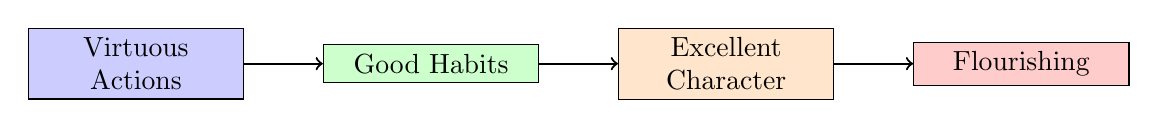
\begin{tikzpicture}[scale=0.9]
    \node[rectangle, draw, fill=blue!20, text width=2.5cm, align=center] (action) {Virtuous Actions};
    \node[rectangle, draw, fill=green!20, text width=2.5cm, align=center, right=of action] (habit) {Good Habits};
    \node[rectangle, draw, fill=orange!20, text width=2.5cm, align=center, right=of habit] (character) {Excellent Character};
    \node[rectangle, draw, fill=red!20, text width=2.5cm, align=center, right=of character] (flour) {Flourishing};
    
    \draw[->, thick] (action) -- (habit);
    \draw[->, thick] (habit) -- (character);
    \draw[->, thick] (character) -- (flour);
\end{tikzpicture}
\end{center}
\end{frame}

% Slide 3
\begin{frame}{Modern Virtue Ethics: Vallor and Haidt's Approach}
\begin{itemize}
    \item Shannon Vallor (philosopher, University of Edinburgh) and Jonathan Haidt (social psychologist, NYU) both apply virtue ethics to modern technology.
    \item They argue that to evaluate technologies like social media and AI, we must ask: "Do these help or hinder human flourishing?"
    \item Both thinkers focus on how technologies shape our character development, especially during crucial periods like childhood and adolescence.
    \item Their approach is \textbf{developmental}: they examine how technology affects our ability to cultivate virtues over time.
\end{itemize}

\begin{table}
\centering
\begin{tabular}{@{}ll@{}}
\toprule
\textbf{Author} & \textbf{Primary Focus} \\ \midrule
Shannon Vallor & Social media ethics and AI's threat to human agency \\
Jonathan Haidt & Social media's impact on childhood development \\ \bottomrule
\end{tabular}
\end{table}
\end{frame}

% Slide 4
\begin{frame}{Why Virtue Ethics for Technology? Beyond Rules and Consequences}
\begin{itemize}
    \item Traditional approaches ask: "Did this violate someone's rights?" (rule-based) or "Did this cause harm?" (consequence-based).
    \item These questions are important, but virtue ethics adds something crucial: "What kind of person is this technology helping me become?"
    \item Technology isn't neutral—it shapes our habits, attention, relationships, and ultimately our character.
    \item A virtue ethics lens reveals how seemingly small technological choices compound over time to fundamentally change who we are.
\end{itemize}

\begin{alertblock}{The Central Question}
Do our technologies help us develop the virtues necessary for human flourishing—or do they undermine our character development?
\end{alertblock}
\end{frame}

% Slide 5
\begin{frame}{The Central Question: Do Our Technologies Help Us Become Good People?}
\begin{itemize}
    \item Vallor and Haidt share a common concern: technology is not just a tool we use, but a force that shapes who we become.
    \item Every time we interact with social media or AI, we are practicing certain habits and reinforcing certain character traits.
    \item The question is not whether these technologies are "good" or "bad" in isolation, but whether they cultivate virtue or vice in us.
    \item Technologies that seem harmless or even beneficial in the short term may undermine our character development over years.
\end{itemize}

\begin{quote}
"The challenge we face today is not a moral dilemma; it is rather a moral imperative, long overdue in recognition, to collectively cultivate the technomoral virtues needed to confront… emerging technosocial challenges wisely and well." — Shannon Vallor
\end{quote}
\end{frame}

% Slide 6
\begin{frame}{The Tower of Babel: Haidt's Metaphor for What Went Wrong}
\begin{itemize}
    \item Haidt uses the biblical story of the Tower of Babel to describe what happened to American society around 2010-2015.
    \item In the story, God confuses the language of people building a tower to heaven, making them unable to communicate or cooperate.
    \item Similarly, social media platforms fragmented our shared reality and made genuine dialogue increasingly difficult.
    \item The result is a society where we inhabit "broken pieces of glass"—isolated echo chambers with no common understanding.
\end{itemize}

\begin{center}
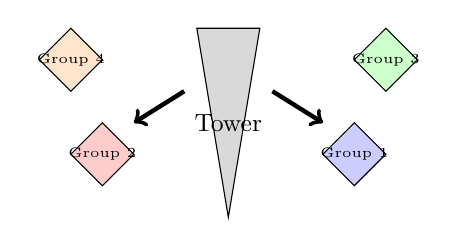
\begin{tikzpicture}[scale=0.8]
    % Tower
    \draw[fill=gray!30] (0,0) -- (0.5,3) -- (-0.5,3) -- cycle;
    \node at (0,1.5) {\small Tower};
    
    % Fragmented pieces
    \draw[fill=blue!20] (2,0.5) -- (2.5,1) -- (2,1.5) -- (1.5,1) -- cycle;
    \node at (2,1) {\tiny Group 1};
    \draw[fill=red!20] (-2,0.5) -- (-1.5,1) -- (-2,1.5) -- (-2.5,1) -- cycle;
    \node at (-2,1) {\tiny Group 2};
    \draw[fill=green!20] (2.5,2) -- (3,2.5) -- (2.5,3) -- (2,2.5) -- cycle;
    \node at (2.5,2.5) {\tiny Group 3};
    \draw[fill=orange!20] (-2.5,2) -- (-2,2.5) -- (-2.5,3) -- (-3,2.5) -- cycle;
    \node at (-2.5,2.5) {\tiny Group 4};
    
    % Arrow showing fragmentation
    \draw[->, ultra thick] (0.7,2) -- (1.5,1.5);
    \draw[->, ultra thick] (-0.7,2) -- (-1.5,1.5);
\end{tikzpicture}
\end{center}
\end{frame}

% Slide 7
\begin{frame}{Vallor's Mirror: AI Reflects Us But Doesn't Think}
\begin{itemize}
    \item Vallor argues that AI systems like ChatGPT are not minds—they are \textbf{mirrors} that reflect human intelligence back at us.
    \item Just as a bathroom mirror shows your face but doesn't have warmth or depth, AI produces \textbf{reflections of intelligence} without understanding or experience.
    \item The danger is not that AI will become conscious and rebel, but that we will mistake these reflections for real thinking.
    \item When we treat AI as a mind, we are tempted to diminish what makes human minds unique and valuable.
\end{itemize}

\begin{block}{Key Distinction}
\textbf{Mind}: Characterized by experience, understanding, consciousness, and meaning-making. \\
\textbf{Mirror}: Reflects the patterns of minds without possessing these qualities itself.
\end{block}
\end{frame}

% Slide 8
\begin{frame}{Agreement: Both Social Media AND AI Threaten Human Flourishing}
\begin{itemize}
    \item Both writers have written extensively on social media (and its harms) before turning to AI in recent years.
    \item Social media undermines our ability to form deep friendships, think critically, and participate in democracy.
    \item AI threatens to make us passive, reducing human agency and our confidence in human judgment.
    \item Both technologies share a common problem: they interfere with the experiences and practices necessary for virtue development.
\end{itemize}

\begin{columns}
\begin{column}{0.5\textwidth}
\textbf{Social Media Problems:}
\begin{itemize}
    \item Fragmented attention
    \item Shallow relationships
    \item Echo chambers
    \item Performative identity
\end{itemize}
\end{column}
\begin{column}{0.5\textwidth}
\textbf{AI Problems:}
\begin{itemize}
    \item Outsourced thinking
    \item Loss of meaning-making
    \item Reduced human agency
    \item Reductive view of mind
\end{itemize}
\end{column}
\end{columns}
\end{frame}

% Slide 9
\begin{frame}{The Timing: Why 2010-2015 Was the Critical Period}
\begin{itemize}
    \item Before 2010, the internet and early social media (Myspace, basic Facebook) did not show negative effects on teen mental health.
    \item Between 2010 and 2015, several technological changes converged: smartphones became ubiquitous, social media added "Like" and "Share" buttons, and algorithms began prioritizing engagement.
    \item This created what Haidt calls \textbf{enhanced virality}—content that triggered strong emotions (especially outrage) spread faster than ever before.
    \item Both authors identify this brief period as when childhood and social life were fundamentally "rewired" across the developed world.
\end{itemize}

\begin{table}
\centering
\begin{tabular}{@{}lll@{}}
\toprule
\textbf{Year} & \textbf{Technology} & \textbf{Impact} \\ \midrule
2007 & iPhone released & Constant internet access \\
2009 & Facebook "Like" button & Quantified social approval \\
2010 & Instagram launched & Visual social comparison \\
2012 & Smartphones reach 50\% of teens & Always-on connectivity \\ \bottomrule
\end{tabular}
\end{table}
\end{frame}

% Slide 10
\begin{frame}{Haidt's Evidence: The Mental Health Crisis by the Numbers}
\begin{itemize}
    \item Between 2010 and 2019, rates of depression and anxiety among U.S. adolescents rose by more than 50 percent in many studies.
    \item The suicide rate for adolescents ages 10-19 rose 48 percent; for girls ages 10-14, it rose 131 percent.
    \item These patterns appeared simultaneously in Canada, the U.K., Australia, New Zealand, and Nordic countries—suggesting a common cause.
    \item Academic performance also declined: after decades of improvement, reading and math scores began dropping globally after 2012.
\end{itemize}

\begin{center}
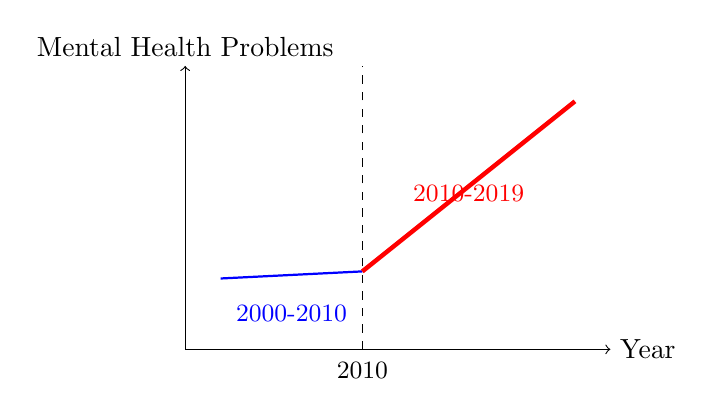
\begin{tikzpicture}[scale=0.9]
    \draw[->] (0,0) -- (6,0) node[right] {Year};
    \draw[->] (0,0) -- (0,4) node[above] {Mental Health Problems};
    
    % Stable period
    \draw[blue, thick] (0.5,1) -- (2.5,1.1);
    \node[blue] at (1.5,0.5) {\small 2000-2010};
    
    % Sharp increase
    \draw[red, ultra thick] (2.5,1.1) -- (5.5,3.5);
    \node[red] at (4,2.2) {\small 2010-2019};
    
    \draw[dashed] (2.5,0) -- (2.5,4);
    \node at (2.5,-0.3) {\small 2010};
\end{tikzpicture}
\end{center}
\end{frame}

% Slide 11
\begin{frame}{Vallor's Evidence: From Social Media to Silicon Valley's AI Dreams}
\begin{itemize}
    \item Vallor's early work (2010s) documented how social media platforms were designed to maximize \textbf{engagement}—keeping users scrolling, clicking, and reacting.
    \item She observed that social media was already promoting a reductive view of human relationships: reducing friendship to "connections" and social life to quantifiable metrics.
    \item More recently, she argues that AI development in Silicon Valley has doubled down on this reductive vision, treating human intelligence as mere "pattern matching."
    \item Both social media and AI embody what she calls the "ideology of efficiency"—measuring everything by optimization and ignoring deeper human values.
\end{itemize}

\begin{alertblock}{The Progression of Concern}
First, social media reduced human relationships to data. Now, AI threatens to reduce human thinking itself to algorithmic processing.
\end{alertblock}
\end{frame}

% Slide 12
\begin{frame}{What Virtues Require: Experience, Practice, and Risk}
\begin{itemize}
    \item Virtues are not abstract principles—they are \textbf{character traits} developed through repeated practice in challenging real-world situations.
    \item To develop courage, we must face genuine fears and risks; to develop practical wisdom, we must make difficult decisions with real consequences.
    \item Friendship requires embodied interaction where we learn to read body language, navigate conflicts, and support each other in person.
    \item \textbf{Civic virtues} like tolerance, compromise, and good judgment require exposure to diverse viewpoints and practice in democratic deliberation.
\end{itemize}

\begin{block}{Three Requirements for Virtue Development}
\begin{enumerate}
    \item \textbf{Experience}: Direct, embodied engagement with the world and others
    \item \textbf{Practice}: Repeated actions that form habits and shape character
    \item \textbf{Risk}: Exposure to genuine consequences that make virtues meaningful
\end{enumerate}
\end{block}
\end{frame}

% Slide 13
\begin{frame}{How Technology Blocks Virtue Development}
\begin{itemize}
    \item Social media and AI systematically remove the three conditions necessary for virtue development: experience, practice, and risk.
    \item Online interactions lack the \textbf{embodied presence} that teaches us to read emotions, navigate conflicts, and build deep trust.
    \item Algorithms optimize for engagement and efficiency, removing the friction and difficulty that force us to develop practical wisdom.
    \item When AI handles our thinking and social media mediates our relationships, we lose opportunities to practice the virtues we need to flourish.
\end{itemize}

\begin{columns}
\begin{column}{0.5\textwidth}
\textbf{What Virtues Need:}
\begin{itemize}
    \item Face-to-face interaction
    \item Genuine consequences
    \item Difficult decisions
    \item Unscripted moments
    \item Real accountability
\end{itemize}
\end{column}
\begin{column}{0.5\textwidth}
\textbf{What Technology Provides:}
\begin{itemize}
    \item Mediated screens
    \item Easy escape/blocking
    \item Algorithmic guidance
    \item Curated feeds
    \item Anonymous actions
\end{itemize}
\end{column}
\end{columns}
\end{frame}

% Slide 14
\begin{frame}{Case Study: Three Generations of Friendship—What Changed?}
\begin{itemize}
    \item \textbf{Grandmother (born 1950s)}: Maintained friendships through weekly letters, occasional long-distance phone calls, and regular in-person visits.
    \item \textbf{Parent (born 1980s)}: Used email and early internet to stay connected, but most friendship activities still happened face-to-face.
    \item \textbf{Teen (born 2008)}: Primary friendship maintenance happens through Snapchat streaks, Instagram comments, and text messages; sees friends in person mainly at school.
    \item The teen has 200+ "friends" online but reports feeling lonely and reports only 2-3 people she could call in a crisis.
\end{itemize}

\begin{block}{Questions to Consider}
Which generation's friendships best cultivated virtues like loyalty, empathy, courage, and practical wisdom? What was gained and lost in each transition?
\end{block}
\end{frame}

% Slide 15
\begin{frame}{Discussion Questions: What Do Friendships Need to Flourish?}
\begin{enumerate}
    \item Haidt identifies four features of real-world interaction that are diminished online: embodied, synchronous, one-to-one, and high-cost communities. Which of these do you think is most important for developing genuine friendship?
    \item Vallor argues that online friendships can be "reflections" of real friendship without the depth of actual friendship. Have you experienced a friendship that felt this way? What was missing?
    \item In the three-generation case study, how might technology have helped each generation maintain friendships? What virtues might have been harder to develop in each era?
    \item If you had to choose: 200 online friends you interact with daily through screens, or 10 close friends you see in person weekly? What does your answer reveal about what you value in friendship?
\end{enumerate}
\end{frame}

% Slide 16
\begin{frame}{Understanding Collective-Action Traps (Why You Can't Just Quit)}
\begin{itemize}
    \item A \textbf{collective-action problem} occurs when everyone would be better off if all took a certain action, but each individual is deterred from acting alone.
    \item Example: Fishermen would all benefit from limiting their catch to preserve fish populations, but any individual who limits their catch just loses money while others overfish.
    \item Social media creates the same trap: most students would prefer if \textit{no one} used Instagram, but each feels they must use it because everyone else does.
    \item In one study, students said they'd need to be paid \$50 to quit Instagram—but would actually \textit{pay} to have everyone quit together.
\end{itemize}

\begin{center}
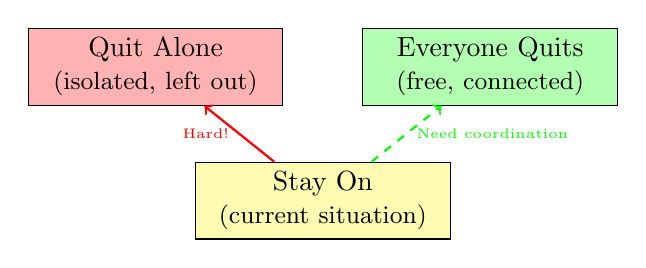
\begin{tikzpicture}[scale=0.85]
    \node[rectangle, draw, fill=red!30, text width=3cm, align=center] (alone) at (0,2) {Quit Alone \\ \small (isolated, left out)};
    \node[rectangle, draw, fill=green!30, text width=3cm, align=center] (everyone) at (5,2) {Everyone Quits \\ \small (free, connected)};
    \node[rectangle, draw, fill=yellow!30, text width=3cm, align=center] (stay) at (2.5,0) {Stay On \\ \small (current situation)};
    
    \draw[->, thick, red] (stay) -- (alone) node[midway, left] {\tiny Hard!};
    \draw[->, thick, green, dashed] (stay) -- (everyone) node[midway, right] {\tiny Need coordination};
\end{tikzpicture}
\end{center}
\end{frame}

% Slide 17
\begin{frame}{Friendship Virtue Lost: The Four Features of Real Interaction}
\begin{itemize}
    \item Haidt identifies four features that characterize healthy human interaction throughout history, all of which are diminished or eliminated online.
    \item \textbf{Embodied}: Real-world interactions use hands, facial expressions, and body language—channels for which we have evolutionary programming that virtual interactions lack.
    \item \textbf{Synchronous}: Real-time interactions teach us conversational turn-taking, timing, and help us feel "in sync" with others in ways that asynchronous texts cannot.
    \item \textbf{One-to-one or one-to-few}: Small-group interactions allow depth and authenticity, while broadcasting to large audiences makes communication performative and anxiety-inducing.
    \item \textbf{High barrier communities}: When exit is difficult, people invest in relationships and repair conflicts; when blocking is easy, relationships become disposable.
\end{itemize}

\begin{block}{The Impact on Virtue}
Without these features, young people develop into adults who are "less comfortable and less skilled at interacting in person"—undermining virtues like empathy, patience, and loyalty.
\end{block}
\end{frame}

% Slide 18
\begin{frame}{Courage and Risk: Why Children Need Dangerous Play}
\begin{itemize}
    \item \textbf{Play} is how young mammals wire their brains—practicing moves and skills they'll need as adults through vigorous, often risky activities.
    \item Children must take risks and fail in environments where failure has real but limited consequences—this is how they overcome fears and learn to estimate danger.
    \item \textbf{Thrilling play} (climbing, rough-housing, exploring unsupervised) appears most effective for overcoming childhood anxieties and building competence.
    \item When children are deprived of risk-taking opportunities, they develop into more anxious, risk-averse adults who struggle with challenges.
\end{itemize}

\begin{quote}
"Young people who are deprived of opportunities for risk taking and independent exploration will, on average, develop into more anxious and risk-averse adults." —Jonathan Haidt
\end{quote}
\end{frame}

% Slide 19
\begin{frame}{Practical Wisdom: "Defend Mode" vs. "Discover Mode"}
\begin{itemize}
    \small
    \item Haidt explains that the brain has two systems: \textbf{approach} (when opportunities beckon) and \textbf{withdrawal} (when threats appear).
    \item People in \textbf{"discover mode"} see the world as full of opportunities—they are happier, less anxious, and more willing to engage with new ideas and people.
    \item People in \textbf{"defend mode"} see the world as full of threats—they are more prone to anxiety, depression, and hostile reactions to others.
    \item Phone-based childhood shifts young people's internal thermostats toward defend mode: constant social comparison, public shaming, and performance anxiety create chronic defensiveness.
\end{itemize}

\begin{center}
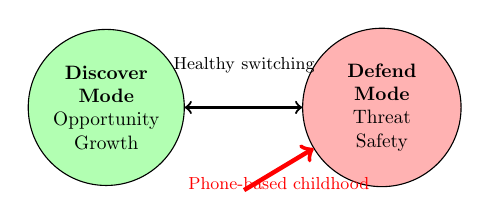
\begin{tikzpicture}[scale=0.7, transform shape]
    % Two modes
    \node[circle, draw, fill=green!30, text width=2cm, align=center] (discover) at (0,0) {\textbf{Discover Mode} \\ Opportunity \\ Growth};
    \node[circle, draw, fill=red!30, text width=2cm, align=center] (defend) at (5,0) {\textbf{Defend Mode} \\ Threat \\ Safety};
    
    % Arrows
    \draw[<->, thick] (discover) -- (defend);
    \node[above, text width=3cm, align=center] at (2.5,0.5) {\small Healthy switching};
    
    % Phone influence
    \draw[->, ultra thick, red] (2.5,-1.5) -- (defend) node[midway, below] {\small Phone-based childhood};
\end{tikzpicture}
\end{center}
\end{frame}

% Slide 20
\begin{frame}{Attention and Temperance: 237 Notifications Per Day}
\begin{itemize}
    \item \textbf{Temperance} is the virtue of moderation and self-control—particularly control over our desires and impulses.
    \item In 2023, the typical adolescent receives 237 notifications per day (roughly 15 every waking hour), each offering "high-pleasure, low-effort digital experiences."
    \item \textbf{Sustained attention} is essential for doing almost anything big, creative, or valuable—but notifications chop attention into fragments.
    \item When students have phone access during class, they use them (especially for texting and social media), and their grades and learning suffer measurably.
\end{itemize}

\begin{table}
\centering
\small
\begin{tabular}{@{}lcc@{}}
\toprule
\textbf{Activity} & \textbf{Requires Sustained Attention?} & \textbf{Compatible with 237 daily pings?} \\ \midrule
Deep reading & Yes & No \\
Creative writing & Yes & No \\
Learning math & Yes & No \\
Solving problems & Yes & No \\
Scrolling TikTok & No & Yes \\ \bottomrule
\end{tabular}
\end{table}
\end{frame}

% Slide 21
\begin{frame}{The Loss of Civic Virtues: Echo Chambers and Spiral of Silence}
\begin{itemize}
    \item \textbf{Civic virtues} are character traits necessary for democratic participation: tolerance, willingness to compromise, ability to deliberate with those who disagree, and intellectual humility.
    \item Social media creates \textbf{echo chambers} (communities of like-minded people who reinforce each other's views) and \textbf{filter bubbles} (algorithmic curation that shows us only what we already agree with).
    \item The "Spiral of Silence" phenomenon intensifies online: people who hold minority or nuanced views stay silent for fear of being attacked by the mob.
    \item Both Vallor and Haidt argue that democracy requires shared reality and genuine dialogue—precisely what fragmented social media undermines.
\end{itemize}

\begin{alertblock}{The Democratic Crisis}
When citizens can't agree on basic facts, can't listen to opposing views, and can't compromise, democracy itself becomes unsustainable. Social media accelerates this fragmentation.
\end{alertblock}
\end{frame}

% Slide 22
\begin{frame}{Haidt's Four Norms for Breaking the Traps}
\begin{itemize}
    \item Because individuals can't escape collective-action traps alone, Haidt proposes four community-level norms that must be adopted together.
    \item These norms are designed to be implemented by parents, schools, and communities working in coordination—not by isolated families acting alone.
    \item Each norm addresses a different aspect of the phone-based childhood problem: devices, platforms, school environment, and real-world alternatives.
    \item Haidt argues that communities adopting all four norms will see substantial improvements in youth mental health within two years.
\end{itemize}

\begin{block}{Haidt's Four Norms}
\begin{enumerate}
    \item \textbf{No smartphones before high school} (age 14)—basic phones only
    \item \textbf{No social media before age 16}—delay account creation
    \item \textbf{Phone-free schools}—locked pouches or lockers during school day
    \item \textbf{More independence, free play, and responsibility}—in the real world
\end{enumerate}
\end{block}
\end{frame}

% Slide 23
\begin{frame}{Case Study: Duckworth's National Survey—Early Findings on School Phone Bans}
\begin{itemize}
    \item Psychologist Angela Duckworth (University of Pennsylvania) is (in 2025-26) leading a national survey called "Phones in Focus" with over 20,000 public school educators responding.
    \item \textbf{Key finding}: "The stricter the policy, the happier the teacher. The stricter the policy, the less distraction there is for students in terms of their academic work."
    \item Teachers report dramatic changes after bell-to-bell bans: students make more eye contact, have more conversations at lunch (instead of "silently scrolling"), and are more engaged in class.
    \item However, only 1 in 4 high schools has a strict ban, compared to 3 in 4 elementary schools—meaning the students who most need support get the least.
    \item Teachers emphasize they face a \textbf{collective-action trap}: individual teachers can't enforce phone policies alone; they need school-wide and district-level support.
\end{itemize}

\end{frame}

% Slide 24
\begin{frame}{Discussion Questions: What Do Students Think About Phone Bans?}
\begin{enumerate}
    \item Duckworth's survey asked teachers and principals, but not students yet. Based on your experience, do you think stricter phone policies would reduce distraction and improve learning? Why or why not?
    \item Teachers report that after phone bans, lunch periods became lively with conversation instead of silent scrolling. Would you see this as a benefit or a loss? What would you miss most about having your phone at lunch?
    \item The research found that high schools have the most lenient policies even though teenagers face the strongest temptations. Do you think this is a mistake, or is there a good reason to trust high schoolers more than younger students?
    \item Teachers said they can't enforce phone rules on their own—they need school-wide support. Have you seen examples of this collective-action trap in your school? What makes it hard for individual teachers to set rules?
\end{enumerate}
\end{frame}

% Slide 25
\begin{frame}{Criticism Corner: Is Haidt Too Anti-Technology?}
\begin{itemize}
    \small
    \item \textbf{Correlation vs. Causation}: Critics note that Haidt shows correlation between smartphone adoption and mental health decline, but correlation doesn't prove causation—other factors (economic anxiety, academic pressure, COVID) might be responsible.
    \item \textbf{Overlooking Benefits}: Some researchers argue Haidt underemphasizes how social media helps isolated teens (LGBTQ+ youth, teens in rural areas, those with disabilities) find community and support.
    \item \textbf{Technological Determinism}: Critics claim Haidt treats technology as an unstoppable force that shapes us, ignoring how people actively choose how to use technology and can develop healthy habits.
    \item \textbf{Impractical Solutions}: Some argue his four norms are unrealistic—parents need to contact kids for safety, teens need phones for logistics, and complete bans might just drive usage underground.
\end{itemize}

\begin{alertblock}{Key Question}
Even if Haidt's data shows correlation and his solutions have challenges, does that mean we should do nothing? What's the appropriate response to preliminary but concerning evidence?
\end{alertblock}
\end{frame}

% Slide 26
\begin{frame}{Transition: From Social Media to Artificial Intelligence}
\begin{itemize}
    \small
    \item Both Haidt and Vallor see social media as undermining human flourishing by fragmenting attention, weakening relationships, and corroding civic virtues.
    \item But in recent years, a new technology has emerged that both authors view as potentially even more threatening: artificial intelligence.
    \item While social media changed how we interact with each other, AI threatens to change how we think, create, and understand ourselves.
    \item Vallor argues that AI presents many of the same dangers as social media (distraction, passivity, reduced human agency) but adds a new threat: the diminishment of what it means to be human.
\end{itemize}

\begin{center}
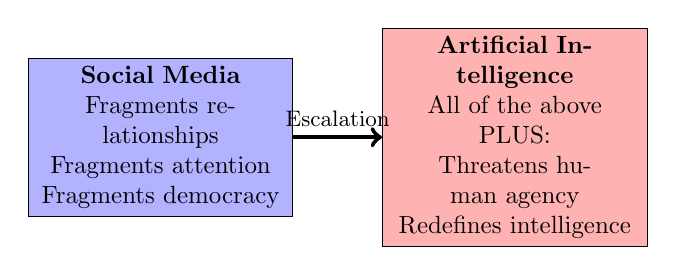
\begin{tikzpicture}[scale=0.9, transform shape]
    \node[rectangle, draw, fill=blue!30, text width=3.5cm, align=center] (sm) at (0,0) {\textbf{Social Media} \\ Fragments relationships \\ Fragments attention \\ Fragments democracy};
    \node[rectangle, draw, fill=red!30, text width=3.5cm, align=center] (ai) at (5,0) {\textbf{Artificial Intelligence} \\ All of the above \\ PLUS: \\ Threatens human agency \\ Redefines intelligence};
    
    \draw[->, ultra thick] (sm) -- (ai) node[midway, above] {\small Escalation};
\end{tikzpicture}
\end{center}
\end{frame}

% Slide 27
\begin{frame}{Why AI Is Not a Mind: The Mirror Metaphor Explained}
\begin{itemize}
    \item When you look in a bathroom mirror, you see a face—but you know there isn't a second person behind the glass with thoughts, feelings, and experiences.
    \item Vallor argues that AI systems like ChatGPT work the same way: they produce \textbf{reflections of intelligence} without actually thinking, understanding, or experiencing anything.
    \item The AI was trained on billions of human texts and learned to produce patterns that \textit{look like} human reasoning, creativity, and knowledge.
    \item Just as a mirror reflection has "no warmth, no depth," AI output lacks the experience, understanding, and meaning-making that characterize genuine thinking.
\end{itemize}

\begin{quote}
"When you go into the bathroom to brush your teeth, you know there isn't a second face looking back at you. That's just a reflection of a face, and it has very different properties. It doesn't have warmth; it doesn't have depth." —Shannon Vallor
\end{quote}
\end{frame}

% Slide 28
\begin{frame}{The Dangerous Myth: "AI Thinks Like Us, But Better"}
\begin{itemize}
    \item Many AI researchers and tech leaders claim that AI systems are developing genuine intelligence and understanding—just like humans, but superior.
    \item This claim is dangerous not (just) because it overestimates AI, but because it \textbf{diminishes what human thinking actually is}.
    \item To make AI seem "intelligent like us," we must reduce human intelligence to mere pattern-matching, prediction, and statistical processing.
    \item Vallor argues this reductive view ignores the most important features of human minds: experience, consciousness, meaning-making, and genuine understanding.
\end{itemize}

\begin{table}
\centering
\begin{tabular}{@{}ll@{}}
\toprule
\textbf{What AI Actually Does} & \textbf{What Humans Actually Do} \\ \midrule
Pattern matching & Genuine understanding \\
Statistical prediction & Creative meaning-making \\
Probability distributions & Conscious experience \\
Optimization & Value-driven judgment \\ \bottomrule
\end{tabular}
\end{table}
\end{frame}

% Slide 29
\begin{frame}{Geoffrey Hinton's Error: Confusing Performance with Understanding}
\begin{itemize}
    \item Geoffrey Hinton won the 2024 Nobel Prize in Physics for pioneering the deep-learning techniques that made modern AI possible.
    \item Yet Vallor argues he makes a fundamental philosophical error when he claims "we understand language in much the same way as these large language models."
    \item Hinton confuses the ability to produce correct outputs (performance) with genuine comprehension (understanding)—like mistaking a calculator's ability to produce "9" for 3+6 with actual understanding of addition.
    \item Because AI can process vastly more data and respond faster than humans, Hinton concludes it might "supplant us" and that "humanity is just a passing phase in the evolution of intelligence."
\end{itemize}

\begin{alertblock}{The Philosophical Mistake}
According to Vallor, Hinton treats \textbf{thinking} as mere information processing, erasing the role of consciousness, experience, and understanding—the very things that make thinking meaningful. What do you think?
\end{alertblock}
\end{frame}

% Slide 30
\begin{frame}{AGI Redefined: From "General Intelligence" to "Replaces Workers"}
\begin{itemize}
    \item \textbf{Artificial General Intelligence (AGI)} originally meant a machine that could do everything a human mind can do—think, understand, feel, create meaning—at human level or better.
    \item Tech leaders like Sam Altman (CEO of OpenAI) have quietly redefined AGI to mean something much narrower: "a system equal to or better than humans at economically valuable tasks."
    \item Under this new definition, AGI doesn't need consciousness, understanding, or meaning-making—it just needs to do your job well enough that your boss can replace you.
    \item Vallor says this redefinition reveals Silicon Valley's values: "Now all we have for the target of AGI is something that your boss can replace you with. It can be as mindless as a toaster, as long as it can do your work."
\end{itemize}

\begin{block}{Two Definitions of AGI}
    \scriptsize
\begin{itemize}
    \item \textbf{Original AGI}: A machine that thinks, understands, and experiences like humans (or better)
    \item \textbf{Redefined AGI}: A machine that performs economically valuable work (regardless of whether it "thinks")
\end{itemize}
\end{block}
\end{frame}

% Slide 31
\begin{frame}{Silicon Valley's Religion: Efficiency as the Highest Good}
\begin{itemize}
    \item Vallor describes Silicon Valley's ideology as having "features of a religion"—certain commitments are "unshakeable by any kind of counterevidence or argument."
    \item The highest value in this worldview is \textbf{efficiency}: accomplishing tasks with maximum speed and minimum friction, regardless of any other considerations.
    \item But efficiency is meaningless without reference to some higher purpose. What is the point of being efficient if not to serve human flourishing?
    \item This ideology leads to viewing intelligence as "a thing that wants to remove the business of thinking"—optimization that eliminates difficulty, ambiguity, and the need for human judgment.
\end{itemize}

\begin{quote}
"It's about achieving a situation where the problem is solved and there's no more friction, no more ambiguity... you've dominated the problem and it's gone and all there is left is your perfect shining solution." —Shannon Vallor
\end{quote}
\end{frame}

% Slide 32
\begin{frame}{The Virtue of Wisdom vs. Mechanical Problem-Solving}
\begin{itemize}
    \item \textbf{Practical wisdom} (or prudence) is the virtue of knowing what matters, what to do in complex situations, and how to live well—Aristotle considered it the master virtue.
    \item Vallor argues there is no "mathematical solution to the problem of justice" because justice involves "conflicting values and interests that cannot be made commensurable on a single scale."
    \item If we allow AI to handle increasingly complex decisions (hiring, medical treatment, criminal justice), we stop practicing the virtue of wisdom and lose confidence in human judgment.
\end{itemize}

\begin{center}
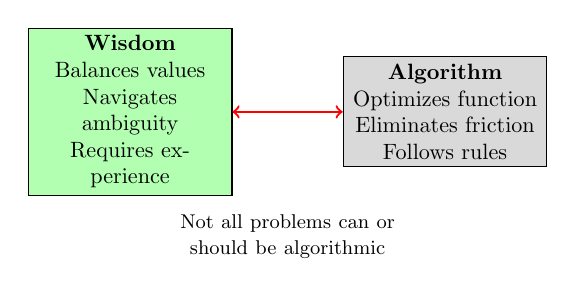
\begin{tikzpicture}[scale=0.8, transform shape]
    \node[rectangle, draw, fill=green!30, text width=3cm, align=center] (wisdom) at (0,0) {\textbf{Wisdom} \\ Balances values \\ Navigates ambiguity \\ Requires experience};
    \node[rectangle, draw, fill=gray!30, text width=3cm, align=center] (algorithm) at (5,0) {\textbf{Algorithm} \\ Optimizes function \\ Eliminates friction \\ Follows rules};
    
    \draw[<->, thick, red] (wisdom) -- (algorithm);
    \node[below, text width=5cm, align=center] at (2.5,-1.5) {\small Not all problems can or should be algorithmic};
\end{tikzpicture}
\end{center}
\end{frame}

% Slide 35
\begin{frame}{Discussion Questions: Vallor on AI and Human Intelligence }
\begin{enumerate}
    \item Vallor uses the mirror metaphor to explain why AI isn't really thinking. Do you find this metaphor convincing? Can you think of ways AI might be more than just a "reflection" of human intelligence?
    \item When Geoffrey Hinton says "we understand language in much the same way as large language models," Vallor says he's confusing performance with understanding. What's the difference? Can something perform perfectly without understanding?
    \item Think about a time you truly understood something (a concept, a friend's feelings, a book). What was that experience like? Could a computer have that same experience by processing the right data?
    \item Silicon Valley leaders redefined AGI from "thinks like humans" to "does economically valuable work." Why does Vallor think this redefinition is dangerous? Do you agree?
\end{enumerate}
\end{frame}

% Slide 37
\begin{frame}{Criticism Corner: Does Vallor Underestimate AI's Significance?}
\begin{itemize}
    \item \textbf{The Existential Risk Camp (e.g., Geoffrey Hinto, Nick Bostrom)}: Some AI researchers argue Vallor underestimates the possibility that AI could develop genuine consciousness or intelligence—and therefore pose existential threats. They worry her "it's just a mirror" view makes us complacent about real dangers.
    \item \textbf{The Techno-Optimists}: Some of these same researchers also believe AI could solve humanity's greatest problems—cure diseases, end poverty, achieve scientific breakthroughs—and that Vallor's focus on current limitations misses AI's transformative potential (for good or ill).
    \item \textbf{The Libertarian Critique}: Some argue Vallor's concerns about Silicon Valley and efficiency reflect a general skepticism toward capitalism and free markets, not specific problems with AI technology itself.
    \item \textbf{The "She'll Be Proven Wrong" Argument}: As AI capabilities advance rapidly, critics suggest her philosophical arguments about AI lacking understanding will seem outdated when systems demonstrate increasingly sophisticated reasoning.
\end{itemize}


\end{frame}

% Slide 38
\begin{frame}{Vallor on Social Media and Democracy: The Fragmented Public Sphere}
\begin{itemize}
    \item Vallor's earlier work extensively examined how social media platforms undermine \textbf{democratic deliberation}—the process by which citizens reason together about shared problems.
    \item Social media creates \textbf{filter bubbles} where algorithms show us only content we already agree with, preventing exposure to diverse viewpoints necessary for democratic citizenship.
    \item The "many-to-many" communication of social media initially seemed liberating, but in practice it enabled mob dynamics, viral outrage, and the spread of misinformation at unprecedented scale.
    \item She argues that democracy requires not just free speech but \textbf{shared reality}—basic agreement on facts—which social media's fragmentation makes nearly impossible.
\end{itemize}

\begin{quote}
"When citizens lose trust in institutions, they lose trust in the stories told by those institutions... young people educated in the post-Babel era are less likely to arrive at a coherent story of who we are as a people." —Shannon Vallor
\end{quote}
\end{frame}

% Slide 39
\begin{frame}{Both Authors on AI: Who Decides What Matters?}
\begin{itemize}
    \item Both Haidt and Vallor worry that AI systems are being designed and deployed by a narrow group of tech leaders with particular values and blind spots.
    \item Haidt notes that AI-powered recommendation algorithms on social media platforms already shape what billions see, read, and believe—concentrating enormous power in few hands.
    \item Vallor argues that if we allow AI to make increasingly important decisions (medical treatment, hiring, criminal justice, education), we're letting \textbf{Silicon Valley's values} (efficiency, optimization, quantification) become society's values.
\end{itemize}

\begin{center}
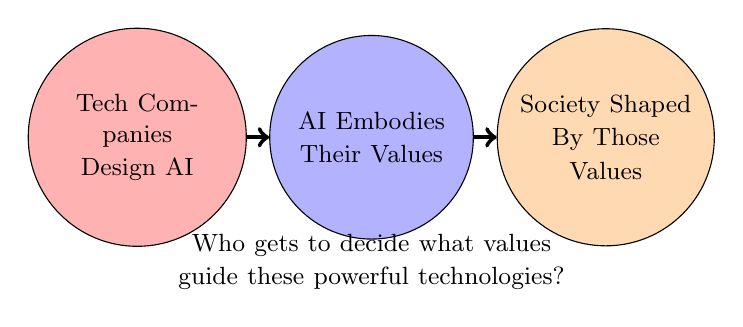
\begin{tikzpicture}[scale=0.85]
    \node[circle, draw, fill=red!30, text width=2.2cm, align=center] (tech) at (0,0) {\small Tech Companies \\ Design AI};
    \node[circle, draw, fill=blue!30, text width=2.2cm, align=center] (values) at (3.5,0) {\small AI Embodies \\ Their Values};
    \node[circle, draw, fill=orange!30, text width=2.2cm, align=center] (society) at (7,0) {\small Society Shaped \\ By Those Values};
    
    \draw[->, ultra thick] (tech) -- (values);
    \draw[->, ultra thick] (values) -- (society);
    \node[below, text width=7cm, align=center] at (3.5,-1.3) {\small Who gets to decide what values guide these powerful technologies?};
\end{tikzpicture}
\end{center}
\end{frame}

% Slide 40
\begin{frame}{Justice Online: Accountability, Doxing, and Cancel Culture}
\begin{itemize}
    \item Both authors grapple with questions of \textbf{justice} in online spaces: When is public shaming warranted? When does it become mob violence?
    \item \textbf{Doxing} (publishing someone's private information online) and coordinated harassment campaigns raise difficult questions about accountability versus cruelty.
    \item Some argue that social media finally enables justice by holding powerful people accountable through public exposure; others see dangerous vigilantism without due process.
    \item The virtue of justice requires both holding people accountable for wrongdoing AND protecting people from disproportionate or wrongful punishment.
    \item Haidt notes that social media makes it easy to "shoot darts" at others with no cost to ourselves, corroding the careful balance that justice requires.
\end{itemize}

\begin{block}{The Justice Dilemma}
How do we maintain accountability for harmful behavior while preserving fairness, proportionality, and the possibility of forgiveness and growth?
\end{block}
\end{frame}

% Slide 41
\begin{frame}{Intellectual Humility: Knowing What You Don't Know}
\begin{itemize}
    \item \textbf{Intellectual humility} is the virtue of recognizing the limits of your knowledge, being willing to revise your beliefs, and acknowledging when others might be right.
    \item Social media undermines this virtue by rewarding confident assertions and punishing admission of uncertainty or error—"I don't know" or "I was wrong" get few likes.
    \item AI systems present themselves with complete confidence even when they're wrong (what researchers call \textbf{hallucinations}), modeling a kind of arrogant certainty.
    \item In a world of infinite information and confident AI, the ability to say "I might be wrong" becomes more important, not less.
\end{itemize}

\begin{table}
\centering
\small
\begin{tabular}{@{}ll@{}}
\toprule
\textbf{Intellectual Humility} & \textbf{Intellectual Arrogance} \\ \midrule
"I could be wrong" & "I'm definitely right" \\
Seeks contrary evidence & Ignores contradictions \\
Updates beliefs & Doubles down \\
Learns from others & Dismisses disagreement \\ \bottomrule
\end{tabular}
\end{table}
\end{frame}

% Slide 42
\begin{frame}{Civic Friendship: Can We Talk Across Differences?}
\begin{itemize}
    \item \textbf{Civic friendship} doesn't mean being best friends with political opponents—it means treating fellow citizens as partners in shared democratic life, not enemies to be destroyed.
    \item Aristotle distinguished three types of friendship: utility (we help each other), pleasure (we enjoy each other), and virtue (we make each other better people).
    \item Civic friendship is closest to utility friendship: we may disagree deeply, but we need each other to make democracy work and to solve shared problems.
    \item Social media corrodes civic friendship by making it easy to dehumanize those we disagree with, to block them entirely, or to performatively attack them for social approval.
\end{itemize}

\begin{alertblock}{The Stakes}
Climate change, pandemics, and economic challenges require cooperation across differences. Without civic friendship, we cannot solve collective problems.
\end{alertblock}
\end{frame}

% Slide 43
\begin{frame}{The Virtue of Community: We Must Act Together}
    \scriptsize
\begin{itemize}
    \item Individual virtue is important, but both Haidt and Vallor emphasize that addressing technology's harms requires \textbf{collective action}—communities working together.
    \item Remember the collective-action trap: what's rational for each individual (staying on social media, using AI) may be harmful for everyone collectively.
    \item Historical examples: neighborhoods organizing to reduce crime, workers forming unions, citizens building public infrastructure—all required community virtue.
\end{itemize}

\begin{center}
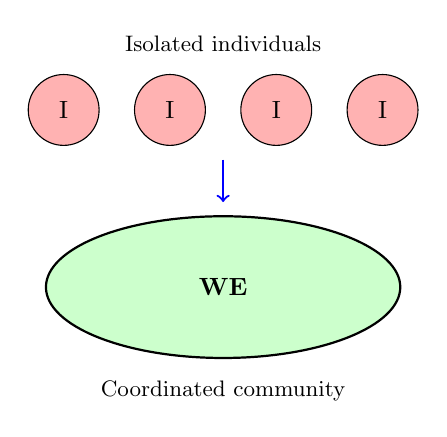
\begin{tikzpicture}[scale=0.9, transform shape]
    \node[circle, draw, fill=red!30, minimum size=1cm] (i1) at (0,0) {I};
    \node[circle, draw, fill=red!30, minimum size=1cm] (i2) at (1.5,0) {I};
    \node[circle, draw, fill=red!30, minimum size=1cm] (i3) at (3,0) {I};
    \node[circle, draw, fill=red!30, minimum size=1cm] (i4) at (4.5,0) {I};
    \node[above] at (2.25,0.7) {\small Isolated individuals};
    
    \node[ellipse, draw, thick, fill=green!20, minimum width=5cm, minimum height=2cm] (comm) at (2.25,-2.5) {};
    \node at (2.25,-2.5) {\textbf{WE}};
    \node[below] at (2.25,-3.7) {\small Coordinated community};
    
    \draw[->, thick, blue] (2.25,-0.7) -- (2.25,-1.3);
\end{tikzpicture}
\end{center}
\end{frame}

% Slide 44
\begin{frame}{Hope: Technology Can Serve Human Flourishing}
\begin{itemize}
    \item Despite their criticisms, neither Haidt nor Vallor wants to eliminate technology or return to a pre-digital world—both see technology's potential for good.
    \item Vallor: "Technology at its core can be as humane an activity as anything can be. We've been technological creatures since before we were \textit{Homo sapiens}."
    \item The question is not "technology or no technology" but "which technologies, designed how, used for what purposes?"
\end{itemize}

\begin{exampleblock}{Virtue-Supporting Tech?}
    \begin{itemize}
        \item Tools that enhance real-world connection (e.g., platforms for community organizing)
        \item AI that augments rather than replaces human judgment (e.g., decision-support systems)
        \item Technologies that promote civic engagement (e.g., tools for deliberative democracy)
    \end{itemize}
    
\end{exampleblock}

\end{frame}

% Slide 46
\begin{frame}{Case Study: Democracy Under Pressure—The 2020 Election and Social Media}
\begin{itemize}
    \item Both Haidt and Vallor point to the 2020 U.S. presidential election as a case study in how social media can undermine democratic civic virtues.
    \item The QAnon conspiracy theory, spread primarily through Facebook, YouTube, and Twitter, convinced millions of Americans of elaborate false narratives—demonstrating social media's power to create alternative realities.
    \item After the election, false claims about voter fraud spread rapidly on social media despite being rejected by courts, election officials, and recounts—fragmenting shared reality.
    \item The January 6, 2021 Capitol insurrection was organized largely through social media platforms, showing how online radicalization translates to real-world violence.
    \item Haidt notes that social media made it "cheap and easy" for foreign actors (like Russia's Internet Research Agency) to "stoke rage on both the left and the right, often over race," further polarizing Americans.
\end{itemize}

\end{frame}

% Slide 47
\begin{frame}{Discussion Questions: What Civic Virtues Does Democracy Need?}
\begin{enumerate}
    \item Both authors argue that democracy requires \textbf{shared reality}—basic agreement on facts. How can a democracy function when citizens live in completely different information universes? Is this situation sustainable?
    \item The 2020 election case shows how social media enables both grassroots organizing and violent extremism. Can we have the benefits (democratic participation) without the harms (radicalization and misinformation)?
    \item Haidt emphasizes \textbf{civic friendship}—treating political opponents as fellow citizens, not enemies. Do you see examples of civic friendship online? What makes it so rare on social media platforms?
    \item Vallor worries that social media discourse trains us to see every disagreement as a battle to win rather than an opportunity to learn. Have you noticed this in yourself or others? How might we cultivate \textbf{intellectual humility} online?
    \item Both authors call for collective action—coordinated responses from communities, not just individual choices. What role should government play in regulating social media to protect democratic virtues?
\end{enumerate}
\end{frame}

\end{document}